% inverted pendulum
\documentclass{standalone}


\usepackage{tikz}
\usetikzlibrary{%
    decorations.pathreplacing,%
    decorations.pathmorphing%
}
\begin{document}
\pagestyle{empty}

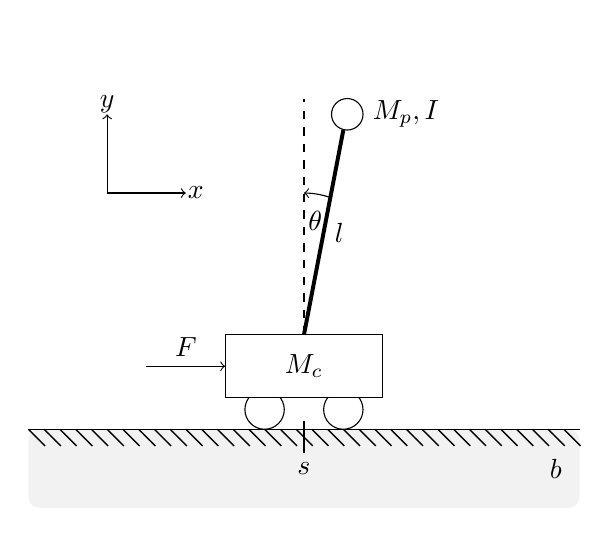
\begin{tikzpicture}[
    media/.style={font={\footnotesize\sffamily}},
    wave/.style={
        decorate,decoration={snake,post length=1.4mm,amplitude=2mm,
        segment length=2mm},thick},
    interface/.style={
        % The border decoration is a path replacing decorator. 
        % For the interface style we want to draw the original path.
        % The postaction option is therefore used to ensure that the
        % border decoration is drawn *after* the original path.
        postaction={draw,decorate,decoration={border,angle=-45,
                    amplitude=0.3cm,segment length=2mm}}},
    ]
    % Road/floor
    \fill[gray!10,rounded corners] (2,-1) rectangle (9,0);
    \draw[black,line width=.5pt,interface](2,0)--(9,0);
    \node at (8.7,-0.5) {$b$};
    
    \fill[white,rounded corners] (2,5) rectangle (9,5.1);
    % car
    \draw (5,0.25) circle (0.25);
    \draw (6,0.25) circle (0.25);
    \fill[fill=white, draw=black] (4.5,0.4) rectangle (6.5,1.2) node[pos=.5] {$M_c$};
    
    % pendulum
    \draw[line width=0.5mm, black](5.5,1.2)--node [right] {$l$}(6,3.8) ;
    \draw (6.05,4) circle (0.2) node[right=2mm] { $M_p,I$};
    
    % force
    \draw[->] (3.5,0.8) --  node [above] {$F$}(4.5,0.8);

     % angle
     \draw [<-,black,domain=90:70] plot ({5.5+cos(\x)}, {2+sin(\x)}) node[left=2mm,below=0.5mm] {$\theta$};
     \draw [dashed] (5.5,1.2) -- (5.5,4.2);
     
     % coordinate system
     \draw[->] (3,3) --  node [right=4mm] {$x$}(4,3);
     \draw[->] (3,3) --  node [above=4mm] {$y$}(3,4);
     
     % position
     \draw(5.5,0.1) --  node [below=2mm] {$s$}(5.5,-0.3);
\end{tikzpicture}


\end{document}